% !TEX encoding = UTF-8 Unicode
\documentclass{beamer}



\usepackage{color}
\usepackage{url}
\usepackage[T2A]{fontenc}
\usepackage[utf8]{inputenc}
\usepackage{graphicx}
\usepackage[english,serbian]{babel}
\usepackage{chemfig}
\usepackage[version=3]{mhchem}
\usepackage{multicol}


\usepackage{hyperref}
\hypersetup{
	colorlinks=true,
	linkcolor=blue,
	filecolor=red,      
	urlcolor=blue,
}

\mode<presentation>
{
  \usetheme{Warsaw} 
  \usecolortheme{default} 
  \usefonttheme{serif}
  \setbeamertemplate{navigation symbols}{}
  \setbeamertemplate{caption}[numbered]
  
} 


\definecolor{mygreen}{rgb}{0,0.7,0}
\definecolor{mygray}{rgb}{0.6,0.6,0.5}
\definecolor{mymauve}{rgb}{0.4,0.1,0.7}

\usepackage{listings}
\lstset{ 
  backgroundcolor=\color{white},
  basicstyle=\scriptsize\ttfamily,
  breakatwhitespace=false,
  breaklines=true,
  captionpos=b,
  commentstyle=\color{mygreen},
  deletekeywords={...},            
  escapeinside={\%*}{*)},          
  extendedchars=true,
  firstnumber=1,              
  frame=single,	                
  keepspaces=true,
  keywordstyle=\color{blue},     
  language=Python,                
  morekeywords={*,...},
  numbers=left, 
  numbersep=4pt,                  
  numberstyle=\tiny\color{mygray}, 
  rulecolor=\color{black},
  showspaces=false,
  showstringspaces=false,
  showtabs=false,
  stepnumber=1, 
  stringstyle=\color{mymauve},
  tabsize=1,
  title=\lstname
}
\usepackage{pgfpages}
\pgfpagesuselayout{resize to}[%
  physical paper width=8in, physical paper height=6in]
\pagenumbering{alph}

\title[\color{gray}Komunikacija preko mreže]{Komunikacija preko mreže:\\izgubljeno poverenje, zavisnost od Interneta}
\author{K.Bakić M.Kovačević N.Milovanović N.Kovačević}
\institute{Matematički fakultet, Beograd}
\date{\today}

\begin{document}

	\begin{frame}
	
	  \titlepage
	\end{frame}

%---: SPISAK TEMA
	\begin{frame}{Sadržaj}
		\tableofcontents 
	\end{frame}
	
	\section{Uvod}
	%prikaz na uskoj plavoj traci
		\begin{frame}{Uvod}
			\begin{itemize}
				\item Internet je globalna mreža koja nam daje mogućnost komunikacije i deljenja resursa na Zemlji. 
				\item Mrežne komunikacije imaju poseban značaj, sve oko nas se pretvara u kompjuter.
				\item Računari i računarske mreže se danas mogu zloupotrebljavati na razne načine.
				\item Javlja se velika zavisnost od Interneta (globalni problem).
			\end{itemize}
		\end{frame}
		%section -----: Iznad, na crnom
	\section{Izgubljeno poverenje}
		\subsection*{Vikipedija}
			\begin{frame}{Vikipedija}
			\begin{itemize}
				\item Vikipediju \textcolor{gray}{(eng. Wikipedia)} doživljavamo kao veliki i bogat skup informacija.
				\item javno je dostupna
				\item više autora može da napiše jedan članak		
				\item nepouzdane informacije	 
				\item izvor informacija može da ostane potpuno nepoznat
				\item Korsgaard i Jensen su 2009. godine predložili promene na softveru.
			 \end{itemize}
			\end{frame}
	
		\subsection*{Internet prevare}
			\begin{frame}{Internet prevare}
				\begin{itemize}
					\item \textcolor{blue}{Pecanje}
						\begin{itemize}
							\item vrsta napada socijalnog inženjeringa
							\item cilj-krađa identiteta korisnika
							\item napretkom tehnologije dolazi do veće rasprostranjenosti
						\end{itemize}
					\item\textcolor{blue}{Nigerijska prevara}
						\begin{itemize}
							\item nastaje oko 1980. godine u Nigeriji
							\item zahteva se pomoć oko transfera novca
							\item Na teritoriji Republike Srbije 2008. i 2009. godine je prijavljeno devet krivičnih dela prevare sa elementima „Nigerijskih prevara“.
						\end{itemize}
					\item \textcolor{blue}{Društvene mreže}
						\begin{itemize}
							\item Fejsbuk, Tviter, Skajp...
							\item \textbf{cilj}: druženje i komunikacija sa prijateljima
							\item\textbf{problemi}: krađe identiteta, svađe, širenje eksplicitnog materijala...
						\end{itemize}
					\end{itemize}
			\end{frame}
			\begin{frame}{Pecanje-primer}
			\begin{figure}[h!]
				\begin{center}
					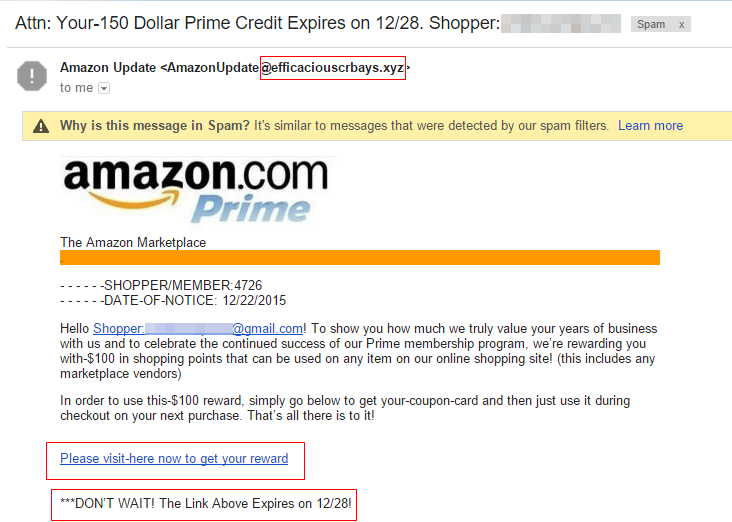
\includegraphics[scale=0.25]{phishing_amazon.png}
				\end{center}
				\caption{Primer pecanja }
				\label{fig:phishing}
			\end{figure}
			\end{frame}
		\subsection*{Masovna kontrola, posmatranje i privatnost na Internetu}
			\begin{frame}{Masovna kontrola, posmatranje i privatnost na Internetu}
			\begin{itemize}
				\item Korisnici Interneta nisu dovoljno svesni koliko podataka o sebi ostavljaju na mreži i u koje svrhe se ti podaci koriste.
				\item Koliko je korišćenje besplatnih servisa na Internetu zapravo besplatno?
				\item \textcolor{blue}{Izdvajaju se dve organizacije sa raznim motivima: }
					\begin{itemize}
						\item Državne organizacije.
						\item Privatne korporacije.
					\end{itemize}
				\item Narušavanje korisničke privatnosti skladištenjem i korišćenjem njihovih privatnih podataka u nemoralne svrhe.
			 \end{itemize}
			\end{frame}

			\subsection*{Državne organizacije}
			\begin{frame}{Državne organizacije.}
			\begin{itemize}
				\item Pravi motivi? Zaštita i sigurnost ili globalna prismotra?
				\item \textcolor{blue}{Primer:} XKEYSCORE, Edward Snowden. Jednostavnim upitom se dolazi do emailova, poruka, HTTP zahteva...
			 \end{itemize}
			 \begin{figure}[h!]
				\begin{center}
					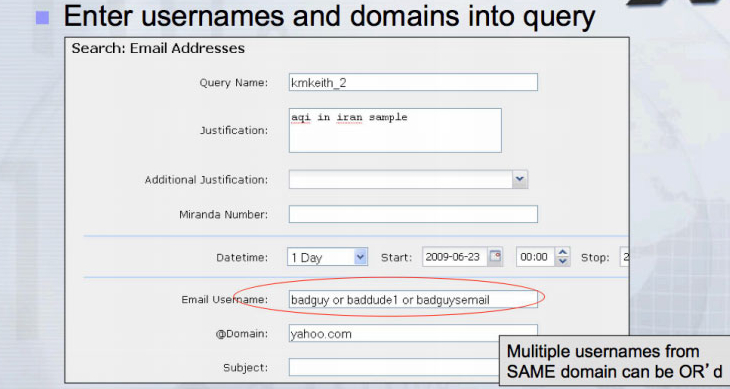
\includegraphics[scale=1.3]{xks.jpg}
				\end{center}
				\caption{Korisnički interfejs XKS} 
			\end{figure}
			\end{frame}
			
			\subsection*{Privatne korporacije}
			\begin{frame}{Privatne korporacije.}
			\begin{itemize}
				\item Proučavanje tržista i iskorišćavanje potreba korisnika (reklame).
				\item Motiv je profit.
				\item Facebook, Google, Youtube, Microsoft, Apple i mnogi drugi.
				\item \textcolor{blue}{Primer:} Eksperiment Facebooka 2012. nad 700.000 ljudi pokazuje da se kontrolisanjem objava koje korisnici vide na početnoj strani može manipulisati njihovim emotivnim stanjima.
			 \end{itemize}
			\end{frame}		
		
	\section{Zavisnost od interneta}
		\subsection*{Prepoznavanje i rasprostranjenost}
		\begin{frame}{Prepoznavanje i rasprostranjenost}
				Prepoznavanje i rasprostranjenost tekst
		\end{frame}
	
		\subsection*{Zavisnost od društvenih mreža}
			\begin{frame}{Zavisnost od društvenih mreža}
				\begin{itemize}
				\item Facebook ima bazu od 2 milijarde mesečnih korisnika, od toga 30\% između 25 i 34 godine
				\item Javlja se potreba za prekomernim korišćenjem društvenih mreža (olakšano pojavom pametnih telefona)
				\item Smanjenje socijalnih i komunikacionih veština
				\item Simptomi slični zavisnosti od hemijskih supstanci (marihuana, kokain, heroin...)
				\item Mišljenja naučnika podeljena u stavu da li ovaj tip zavisnosti treba klasifikovati kao poremećaj
				\end{itemize}
			\end{frame}
		\subsection*{Zavisnost od Internet igara}
		\begin{frame}{zavisnost od Internet igara}
		\begin{itemize}

			\item Razvojem Interneta uporedo se razvijaju razni tipovi PC igara kojima je neophodna konekcija na internet (MMORPG, MOBA...)
			\item Osobe sa dva kraja planete mogu da igraju igru u isto vreme
			\item Predstavljaju idealan beg od sveta
			\linebreak
			\item Problem su, takodje, igre na sreću
			\item Zbog loše zaštite stranica, mogu da im pristupe i deca mlađa od 18 godina
		\end{itemize}			
		\end{frame}
		
		\begin{frame}{Primer}
		\begin{figure}[h!]
			\begin{center}
				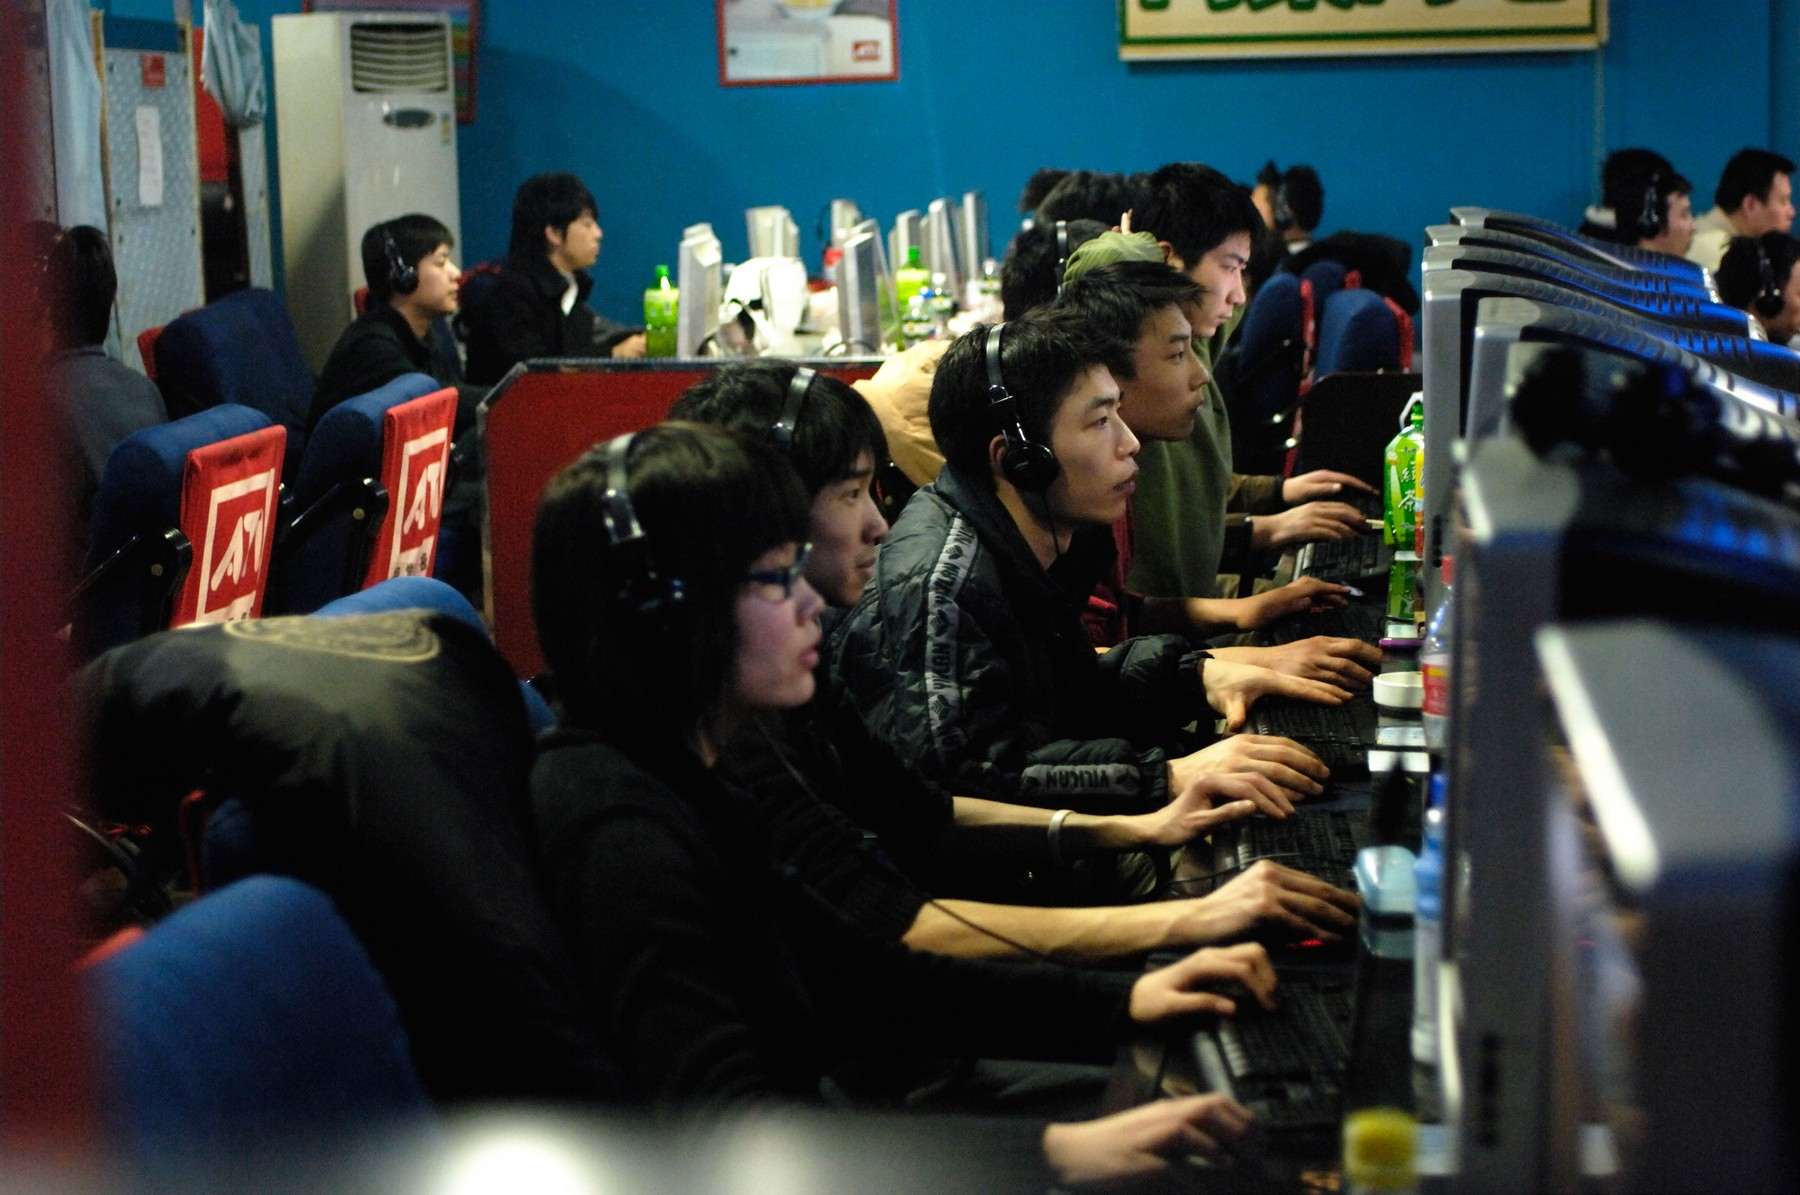
\includegraphics[scale=0.15]{internet_cafe.jpg}
			\end{center}
			\caption{Internet cafe}
			\label{fig:zavisnost}
		\end{figure}
		
		\end{frame}
		
		\subsection*{Posledice}
		\begin{frame}{Posledice}
			Posledice tekst
		\end{frame}
		
	
	\section{Literatura}
		\begin{frame}{Literatura}
		%	\bibliography{seminarski} 
			\begin{itemize}
				\scriptsize
				\item Bruce Schneier, Data and Goliath (2015)
				\item Evgeny Morozov, The Net Delusion: The Dark Side of Internet Freedom (2011)
				\item Glenn Greenwald, No Place to Hide: Edward Snowden, the NSA, and the U.S. Surveillance State (2014)
				\item Jelena Matijasević, Žaklina Spalević, Vrste internet prevara-pojam,značaj i uticaj na ekonomske i moralne aspekte društvene zajednice (2012)
				\item Mudasir Ahmad Wani, Suraiya Jabina, A sneak into the Devil’s Colony- Fake Profiles in Online Social Networks (2017)
				\item Statista, Social networks ranked by number of users (2019)
				\item Teun Lucassen, Trust in Online Information (2013)
				\item Turkle, Sherry, Alone together: Why we expect more from technology and less from each other (2017)
				
			\end{itemize}
			\bibliographystyle{unsrt}
		\end{frame}

\end{document}
